
\chapter{Introduction }
\label{ch:Chapter1}
%\section{Introduction}
%Para-1 - What are safety-critical cps? Some egs. of their existance in different applications. What are the damages they are capable of causing?
\ac{CPS} combine the cyber capabilities with physical capabilities which neither part can solve alone \cite{Platzer18}. %They are useful in multiple application domains \cite{10.1145/2038642.2038685}\cite{10.1145/1837274.1837463} \cite{6051465}.
Some common safety-critical applications include medical devices \cite{10.1145/2038642.2038667} \cite{6051465} \cite{10.1145/2461328.2461369} \cite{Bresolin2015} % \ag{you might want to not put too many references for the examples. Consider focusing on putting references related to the concepts that you will utilize or have seen wrt the topic of the paper}.
Unfortunately, there have been multiple, targeted attacks on safety-critical CPS such as pacemakers\cite{4531149}, airplanes \cite{217595} etc.  %cars \cite{10.5555/1929820.1929848},   %drones and rovers \cite{10.1145/3359789.3359847}. 

%\todot{Add some more examples from practical world to show the importance of safety-critical world} Hence, they require hard guarantees otherwise they can lead to incomprehensible damages such as loss of life. There have been reports where self-driving cars ended up in crashes leading to loss of life. \todot{Add some real life examples of damage due to reliability}

%Paragrah-2 - controller based cyber physical systems - What have cps been modelled using previously and the different sort of attacks that have been show in those cases. 
Traditionally, CPS have used classical control theory-based controllers  \cite{1337806} \cite{10.1145/2038642.2038667} \cite{6051465}. Control theory utilizes differential equations to model the systems' behavior, while accounting for any external factors that might affect the system e.g., friction, wind etc. This makes them vulnerable to malicious attacks that exploit these tolerances.
%The first publicly reported targeted attack on a SCADA system \cite{article22} was the attack on Maroochy Shire Council’s sewage control system in Queensland, Australia where the attacker caused more than 750,000 gallons of untreated sewage water to be released into parks and resulted in more than \$200,000 clean up damages \cite{10.1016/j.adhoc.2009.04.012}. There have also been targeted attacks demonstrated on surgical robots \cite{7579758}, bugs disguised as attacks \cite{242054}. There have been multiple attacks to the control systems in the past but a lot of the attacks have no public information\cite{doi:10.1080/13518040590969785}
%\todot{Add more examples of attacks here from papers}
%

%Paragraph 3- What are FDI attacks? - why are they common? - previous instances of these attacks. 
For example, by targeting the way sensors capture real-world data, an attacker can inject a false sensor reading. These are called \ac{FDIA}. In an FDIA, an attacker compromises the measurements from the sensors in such a way that undetected errors are introduced in the outputs by changing the state estimation \cite{7438916}. In turn, these can lead to incorrect actions or unintended behavior. 
%The change in the state estimation leads to a wrong step being taken by the system.  


%paragraph 4- What are DNN based controllers? Why are they being used in CPS? Why is this work important?

Recently,  \ac{DNN} based controllers are replacing classical control-theory based controllers \cite{xiang18} \cite{Kocic2019} \cite{bechtel2017deeppicar}. There are two reasons for using DNNs in CPS: %\ag{you might want to use \textit{itemize/enumerate} to properly format the points. Might become difficult for the reader} 
1) due to the data-based nature of DNNs, modeling the systems is easier as compared to control theory based systems, which require domain expertise \cite{Aamir_2013}, 2) modeling complex CPS such as autonomous vehicles has certain limitations when using classical control theory \cite{article23}. For example, autonomous vehicles require multiple interacting dynamic control systems, whereas conventional control designs are built for only one specific system. DNNs provide this dynamic capability.

%There are two types of FDIA: random FDIA and targeted FDIA. 
%To construct a targeted FDIA, the relationship described through classical control theory is assumed to be known by the attacker. Hence, previous techniques proposed for targeted
FDIA generation techniques for classical control theory based controllers \cite{10.1145/1952982.1952995} are not applicable to DNNs because they have different mathematical representations. This is because typical FDIA techniques construct attack vectors according to the control-theory equations. %In DNN these equations are different and the same attack vectors cannot be used.
% since the interfaces are completely different. 
Further, in classical control theory, small perturbations in specific inputs can lead to changes in outputs by changing the state estimations. %There have been multiple mechanisms proposed to synthesize the FDIA in classical controllers.  
However, using the same mechanisms to synthesize FDIA in DNN  based controllers as stated above does not work as said above %due to the differences in their interface \ag{This statement is mentioned at the start of the paragraph, just in different words. Consider why this sentence is different}
-- we design a technique to synthesize FDIA for DNN controllers. We call these \attack as they are transmitted through the DNN's layers in the CPS like ripples in large puddle of water. % \karthik{How do ripple attacks differ from classical FDIAs? - they are transmitted through the layers, unlike in classical fdia since there are no layers type structure in control theory.}

%paragraph 3a
A ripple is created when the perturbation caused at the input layer is transmitted to the output layer thereby causing deviations without raising any alarms. 
%However, to cause a successful ripple it is important to identify the  input and its perturbation that will ensure that the output is deviated by a certain threshold. %If we conduct a FDI attack but by perturbing the not so effective input \karthik{What does this mean}, the ripple will not be successful. Hence, t
To mount a successful \attack, we need to identify two things: 1) the critical inputs-- these are inputs that affect the final outputs most on being perturbed; inputs most likely to generate a ripple in the network and , 2) the smallest amount by which each critical input needs to be perturbed to cause a ripple. We are looking for the smallest perturbations because large deviations in the inputs can trigger alarms due to the inbuilt error detection mechanisms that 
check the upper and lower bounds of the inputs to prevent them from deviating by large amounts.
%\karthik{I don't understand the difference}
%\karthik{This is the same point as the one above}. DNNs are constructed using data that provides an input-output mapping for the controller. \karthik{So what?}


In this work, we ask whether { \attack \em can be mounted on DNN-based controllers, and if so, whether it is possible to find the attacks automatically with minimal cost.} 
%karthik{Doesn't automatic imply minimal effort ? Did you mean cost ?}. - yes cost  }
%since mathematical modeling is different. \karthik{So I'm not sure I understand why this is specific to control theory ?}
%The traditional FDIA has been conducted in a control theory based CPS settings. 
%We introduce similar FDIA attacks in our work called drift attacks that cause the inputs to drift over time eventually leading to some bad outcome. These attacks are conducted on Deep Neural Network(DNN) based CPS.  

%Due to the advancements in DNN in the recent years, there are some realistic cases of self-driving cars visible these days. There has been a lot of work that focuses on modeling CPS using DNNs in different settings  
%In this paper, we address the question - \textit{Are DNN based CPS subject to FDIA, and if so, what is the effort required to conduct such attacks?} 
%\karthik{What mechanisms are these?- yes done}.  	
%Paragraph 4a - why is the FDIA in DNN be challenging?

To synthesize ripples in DNN based CPS, there are two main challenges. First, the state space for DNN based systems is very big since the DNN model is constructed using huge data sets. This makes it difficult to find the perturbations for inputs. If an attacker is conducting the attack in a practical setting, she has limited time to mount the attacks.  %\karthik{Why is limited time a factor?}. 
Second, the existence of non-linear activation functions such as ReLU makes it difficult to find linear mappings between the inputs and the outputs to synthesize \attack.
%\karthik{Does ripple mean just the perturbation or does it include the input?}.                                                            

%To understand the the existance of successful ripples in DNN based CPS, there are two challenges with respect to the control theory approach. First, the state space for DNN based systems is typically much bigger than control-theoretic models. The reason behind this is that the control theory equations are well defined for different different modes for state estimation. In DNNs, this is not the case, since the model is defined using the data-set, and needs to capture the behaviors for the CPS. %\karthik{Really ? All possible behaviors ?}. 
%Therefore, verification of DNNs is still an open and challenging problem. Researchers have spent a lot of time on verifying the properties for CPS modeled using control theory using theorem proving \cite{Araiza_Illan_2014} \cite{SYS-001} . Hence, there are guarantees associated with the control theory systems. However, DNNs lack in providing strong guarantees for the systems due to the reasons stated above. 
%Second, DNNs are non-linear in nature due to the introduction of activation functions at each layer that determine the output for the neural network. There are multiple non-linear activation functions such as Sigmoid, tanH, ReLU and many others\cite{Goodfellow-et-al-2016}. 
%Figure 1. is the ReLU function which we use for our work%\karthik{What's the point of this figure?}. 

%To generate the FDIA, we focus on one type of non-linear activation function which is the Rectified Linear Unit (ReLU). The adoption of ReLU is considered as one of the milestones in deep learning revolution since the technique permits very deep neural networks ~\cite{Goodfellow-et-al-2016}.
%The reason we specifically chose ReLU for our tool is because as shown in Figure 1 , it can be partitioned to be represented in a piece-wise linear format. This property and the structure of the DNNs allows us to model it in Mixed-Integer Linear Programming (MILP) format. Mixed Integer Linear Porgramming (MILP) allows us to create models to find feasible solutions for the models. In our case we create a DNN model such that we can find security attacks using our formulation.     \karthik{We haven't introduced this yet? - AK(DOne)}

Our technique tackles both the challenges and finds the critical inputs and also the minimal perturbations to cause a successful \attack. To do so, we model the attack synthesis as an optimization problem using\ac{MILP}, and build an automated tool called \tool. %to find \attack \ag{You can end the sentence at \tool} .

To tackle the state space explosion, we design \attack specific cost functions (i.e., objective functions) that reduce the search space significantly. This allows us to efficiently find the ripples (if they exist), or provide a proof of their absence in that specific setting. To find the smallest perturbations that cause  ripples, we define the model as a set of equations and constraints with an objective function. Therefore, finding the perturbations is achieved by solving the model. Minimizing cost functions provides an assurance that the smallest possible perturbations are found. %\karthik{Why is this important? Who's we here ? - It is imp because smallest perturbation means minimal effort from attacker}. %The next approach \karthik{What's the first approach ? I've told  you before - say upfront how many approaches you have and label them} 
Further we also locate the critical inputs automatically. Instead of trying to perturb all the inputs in a system, we focus on perturbing only the critical %\karthik{Is this the same as the critical input? Be consistent in terminology -yes}
inputs as it significantly reduces the search space and the time taken to synthesize the attacks %\karthik{I don't understand - I thought you already found the ripples - yes but ripples can exist by  perturbing multiple inputs and/or one input, the ripples that exist sucessfully with perturbing even a single input are called critical inputs.}. 

We handle the non-linearity of activation functions in two ways. First, we chose the ReLU activation function as this can be converted from a non-linear function to a piece-wise linear function by adding a set of logical constraints. This allows us to create solvable models in MILP. Second, we add constraints to bound the search space that allows \tool to return results without state-space explosion. %\karthik{What's the second thing?}
%\karthik{Wait a second - you just said it was non-linear, but now you're saying it's piece-wise linear}

%\begin{figure}
%	\centering
%	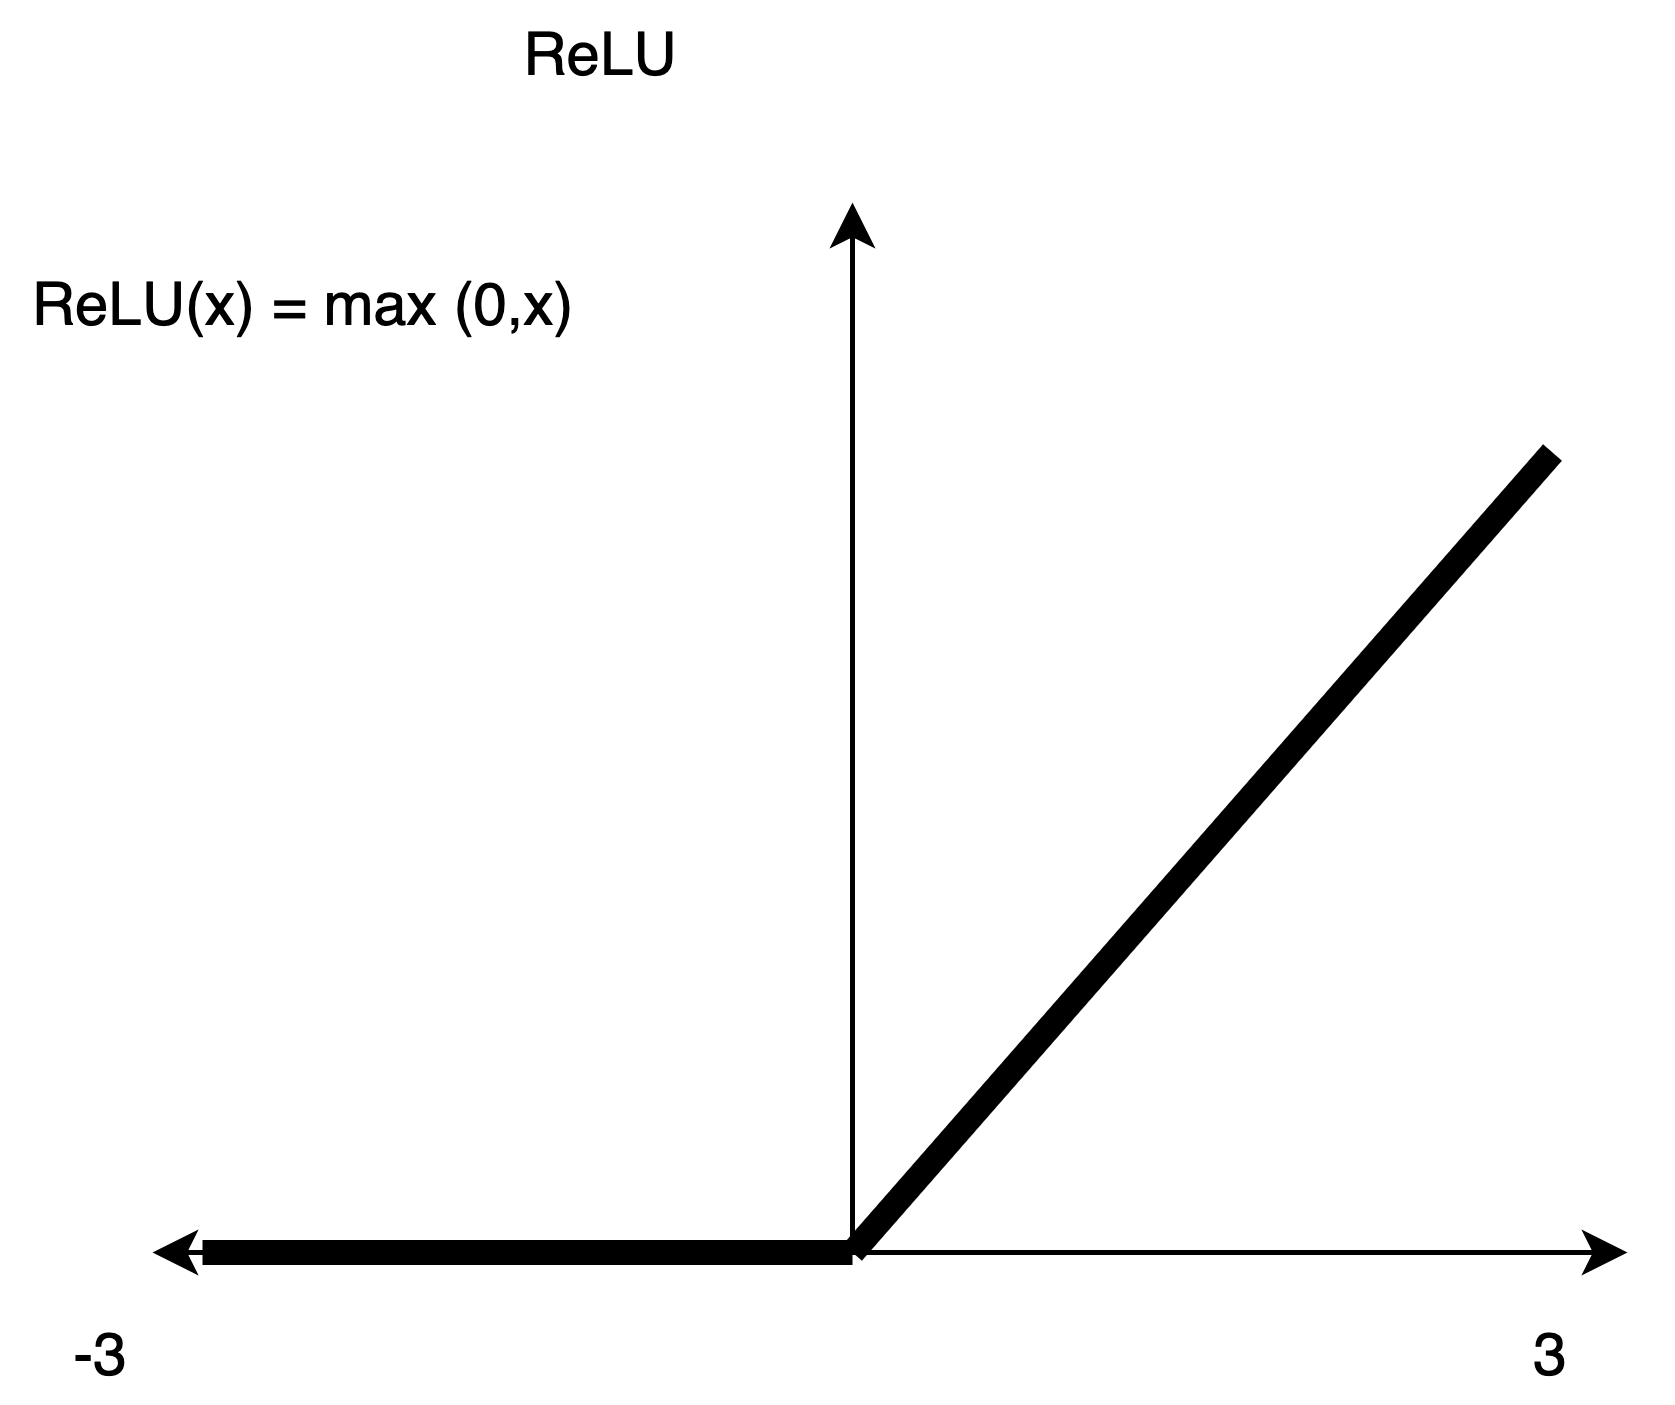
\includegraphics[width=0.7\linewidth]{Images/ReLU}
%	\caption[Activation functions]{ReLU activation function}
%	\label{fig:ReLU}
%\end{figure}


% Paragraph 5 - Building up on the non-linearity challenge 1) why are relu being used so much 2) what is relu doing
%The ReLU activation function is computationally efficient and allows the network to converge very quickly. \karthik{I don't understand the relevance of this statement} 
%The ReLU is a function that returns the value provided for the positive values or the value zero if the input is negative as shown in Figure 1. This shows that ReLU is piece-wise linear and we leverage this property to model the DNN as an optimization problem to generate FDIA. \karthik{Can you please be more direct about what your insight here is? Is it that we can take a non-linear function and make it piece-wise linear?}
%\todot{Explain more about the non-linearity and CPS connections here}
%\karthik{What's the first observation?- relu was the first observation, but now i have changed the paragraph}
%After building a MILP model to conduct a successful ripple attack, we find that perturbing one input is enough to cause an output change without triggering alarms. The reason this happens is that there are some inputs which we call as the critical inputs, carry more weight than the others and if perturbed by certain values can cause damage by taking the wrong decision . Our tool not only allows us to find these inputs but also find the minimum perturbations that can lead to a ripple.  \karthik{You need to explain why this is the case - AK (done)} 

%Hence, to find those specific critical inputs in which perturbations cause damage in DNN based CPS, we use MILP. \karthik{Again, not clear what this has to do with MILP}
%Using MILP provides a significant (about 10x) improvement over brute force approaches to find the critical inputs that cause damage.    \karthik{Now why are we discussing the results here}\aarti{i dont know}

%Para 6/Problem statement
%\karthik{Lot of acronymns below without expansions}
%There has been work that models the DNNs in SMT solvers \cite{10.1007/978-3-319-63387-9_5}, or MILP encodings \cite{10.1145/3302504.3313351} to find the upper and lower bounds in DNNs. These techniques find the general upper and lower bounds for the DNNs which do not provide us hard guarantees for every state. These techniques try to explore every possible input-output combination possible in the space. This does not scale because of the complexity of the DNNs, and therefore leads to state explosion \karthik{Cite}. 
%Also, providing general upper and lower bounds does not show that the systems are free of side channel attacks or stealthy attacks such as the FDIA \karthik{Why are we talking about side-channel attacks?}. There have been many attacks on DNN systems that uses adversarial perturbations in the inputs for mis-classifying outputs \cite{Szegedy2013IntriguingPO}\cite{deng2020analysis}. %\karthik{Provide citations}
%However, there is no work or automated technique that demonstrates FDI attacks in DNN based controllers for CPS. 
%Also, it is not a trivial task to map the existing techniques directly since our use case is different from the previous use-cases. 
{\textit{To the best of our knowledge, we are the first to  propose an automated approach to systematically locate the critical inputs and find the minimum perturbations to conduct a \ac{RFDIA} for DNN-based controller systems.}}
%{\textit{To the best of our knowledge, we are the first to systematically propose security optimizations to find the optimal FDI attacks for DNN based controllers for CPS by finding the critical inputs instead of perturbing all the inputs. }
%\todot{Frame the problem statement better}
\newline
%Main contributions of the work
The main contributions in this paper are as follows:
%\setlist{nolistsep}
\newline
\begin{enumerate}
	\item Demonstrate that FDIA on classical control-theory based CPS are also applicable to DNN-based controllers, and define RFDIA specific to DNN based CPS. %\ag{Didnt you mention that FDIA for control-theory based CPS is not applicable to DNN-based CPS? Which is what this paper addresses about?- attacks are applicable; attack generation technique is not} 
	% \karthik{How can you abstract the system as a problem?}
	% \newline
	\item Model the attack synthesis as an optimization problem (specifically as a MILP). %\karthik{Once you define an acronymn, use it consistently} 
	%to build a query like mechanism for conducting ripples.  %\karthik{such as?} 
	%  \item We discuss our key insights in selecting the automated techniques for our use-case. 
	%\newline
	
	\item Implement a tool called \tool, and demonstrate its applicability by synthesizing \attack.%\karthik{Make this a macro in latex} 
	\item Using \tool, we successfully identify the \textit{critical inputs} in three important safety-critical applications: \ac{APS},  and  two collision avoidance systems for unmanned vehicles called \ac{ACAS-Xu} and \ac{HCAS}.
	\item Evaluate \tool's performance and show that it can synthesize \attack in a short time period.   % and utilizing limited memory. 
	%\karthik{What about memory ?- very less memory - it can also run on rpi given gurobi can be easily installed on it.} 
	%\newline
\end{enumerate}

% Karthik - I folded this in with the contributions above- pk
%Our evaluation shows that ReLUSyn can provide a uniform platform for finding security attacks in a complex system constructed using DNNs. ReLUSyn also shows that we can abstract the security problem as an optimization problem to systematically find the possible attacks in the form of FDI and reason about the system. We believe we are the first to propose an optimization framework that allows different attack modeling for DNNs. We show modelings for three types of FDI attacks. SInce the framework comes with three predefined attack models they can utilise them directly. We also believe this will lead to future work as researchers can model their own attacks for their applications and use the framework. This provides a plug and play functionality within our framework. 

%ReLUSyn always returns a result if there is a FDI attack possible \karthik{Can we use terms such as sound, complete etc.?}. It also allows us to find more subtle perturbations to conduct the FDI attacks by applying specific optimizations while modeling the DNN using MILP \karthik{I don't understand}. We demonstrate three different attacks for two different applications of CPS, and hence, in the future designing more cost functions for different attacks can be a way to proceed towards the ideal case \karthik{What ideal case ?}. 

%The goal of ReLUSyn is to identify the critical inputs that on perturbing cause changes in the outputs. 

%These attacks can lead to safety violations such as wrong amounts of insulin being injected in a patient, and crashes in a collision avoidance systems. 
% \karthik{Say something about the consequences of the attacks found}
%\karthik{Which ones -done} 
% Identification of critical inputs allows \tool to synthesize \attack efficiently %\karthik{So you can't synthesize them otherwise? - it will just take more time. focusing with the critical inputs approach allows us to understand the nature of the DNN and which inputs carry more weight. It is just interesting to know that. }. %We call these attacks as ripple attacks because with small changes in the inputs get carried over through the layers till the end and their effects can be observed in the output layer. \karthik{Did't we say this already ? Why do you keep repeating the same thing ?}
% Furthermore, \tool  provides a significant (about 10x)  improvement %\karthik{Of what?} 
%over brute force approaches in the time taken to conduct a \attack. \ag{do you test the brute force approach too? Mention in brief about that if not} 
%\karthik{Ithought you said brute force doesn't generate attacks at all?}
%\karthik{For heaven's sake, be consistent in terminology ! Is it ripples, or ripple attacks ?}   %\karthik{Talk about brute force comparison here-done}
%We demonstrate our attacks on three safety-critical systems ACAS Xu, HorizontalCAS and APS DNN. 
%We provide a systematic approach to find the inputs in order to compromise the system by utilising the physical notion of CPS and the DNN centric modelling. 
%In the next section we provide our problem formulation with the background. We follow this section with a motivating that we use to explain challenges in the next section. This is followed by the related work and the methodology. We finally present our results in the section followed by the methodology. 

